\documentclass[11pt,a4paper,twoside,openright]{report}

\usepackage[top=25mm,bottom=25mm,right=25mm,left=30mm,head=12.5mm,foot=12.5mm]{geometry}
\let\openright=\cleardoublepage

\usepackage[a-2u]{pdfx}

\usepackage[
   backend=biber
%  ,style=iso-authoryear
  ,style=alphabetic
  ,citestyle=numeric
  ,sortlocale=cs_CZ
  ,bibencoding=UTF8
  %,block=ragged
]{biblatex}
\addbibresource{references.bib}

%% Přepneme na českou sazbu, fonty Latin Modern a kódování češtiny
\usepackage[czech]{babel}
\usepackage{lmodern}
\usepackage[T1]{fontenc}
\usepackage{textcomp}
\usepackage[utf8]{inputenc}

% Set fonts
\RequirePackage[osf]{mathpazo} % Palatino with oldstyle figures
\newcommand\liningnums[1]{\fontfamily{ppl}\selectfont#1}
\RequirePackage{eulervm}
\RequirePackage[scaled=.8819]{sourcecodepro} % Source Code Pro typeface for monospace

%%% Další užitečné balíčky (jsou součástí běžných distribucí LaTeXu)
\usepackage{amsmath}        % rozšíření pro sazbu matematiky
\usepackage{amsfonts}       % matematické fonty
\usepackage{amsthm}         % sazba vět, definic apod.
\usepackage{bm}             % tučné symboly (příkaz \bm)
\usepackage{graphicx}       % vkládání obrázků
\usepackage{fancyvrb}       % vylepšené prostředí pro strojové písmo
\usepackage{fancyhdr}       % prostředí pohodlnější nastavení hlavy a paty stránek
\usepackage{icomma}         % inteligetní čárka v matematickém módu
\usepackage{dcolumn}        % lepší zarovnání sloupců v tabulkách
\usepackage{booktabs}       % lepší vodorovné linky v tabulkách
\makeatletter
\@ifpackageloaded{xcolor}{
   \@ifpackagewith{xcolor}{usenames}{}{\PassOptionsToPackage{usenames}{xcolor}}
  }{\usepackage[usenames]{xcolor}} % barevná sazba
\makeatother
\usepackage{multicol}       % práce s více sloupci na stránce
\usepackage{caption}
\usepackage{enumitem}
\usepackage{lipsum}
\setlist[itemize]{noitemsep, topsep=0pt, partopsep=0pt}
\setlist[enumerate]{noitemsep, topsep=0pt, partopsep=0pt}
\setlist[description]{noitemsep, topsep=0pt, partopsep=0pt}
\usepackage{pdfpages}

\usepackage{tocloft}
\setlength\cftparskip{0pt}
\setlength\cftbeforechapskip{1.5ex}
\setlength\cftfigindent{0pt}
\setlength\cfttabindent{0pt}
\setlength\cftbeforeloftitleskip{0pt}
\setlength\cftbeforelottitleskip{0pt}
\setlength\cftbeforetoctitleskip{0pt}
\renewcommand{\cftlottitlefont}{\Huge\bfseries}
\renewcommand{\cftloftitlefont}{\Huge\bfseries}
\renewcommand{\cfttoctitlefont}{\Huge\bfseries}

% vyznaceni odstavcu
\parindent=0pt
\parskip=11pt

% zakaz vdov a sirotku - jednoradkovych pocatku ci koncu odstavcu na prechodu mezi strankami
\clubpenalty=1000
\widowpenalty=1000
\displaywidowpenalty=1000

% nastaveni radkovani
\renewcommand{\baselinestretch}{1.20}

% nastavení hlavy a paty stránek
\fancyhf{}
\renewcommand{\chaptermark}[1]{\markboth{#1}{}}
\fancyhead[RO,LE]{\leftmark}
\fancyfoot[RO,LE]{\thepage}
%\renewcommand{\footrulewidth}{0pt}
\fancypagestyle{plain}{%
\fancyhf{} % clear all header and footer fields
\fancyfoot[RO,LE]{\thepage}
\renewcommand{\headrulewidth}{0pt}
%\renewcommand{\footrulewidth}{0.5pt}
}

% Tato makra přesvědčují mírně ošklivým trikem LaTeX, aby hlavičky kapitol
% sázel příčetněji a nevynechával nad nimi spoustu místa. Směle ignorujte.
\makeatletter
\def\@makechapterhead#1{
  {\parindent \z@ \raggedright 
   \Huge\bfseries \thechapter. #1
   \par\nobreak
   \vskip 20\p@
}}
\def\@makeschapterhead#1{
  {\parindent \z@ \raggedright 
   \Huge\bfseries #1
   \par\nobreak
   \vskip 20\p@
}}
\makeatother

% Trochu volnější nastavení dělení slov, než je default.
\lefthyphenmin=2
\righthyphenmin=2

% Zapne černé "slimáky" na koncích řádků, které přetekly, abychom si
% jich lépe všimli.
\overfullrule=1mm

%% Balíček hyperref, kterým jdou vyrábět klikací odkazy v PDF,
%% ale hlavně ho používáme k uložení metadat do PDF (včetně obsahu).
%% Většinu nastavítek přednastaví balíček pdfx.
\hypersetup{unicode}
\hypersetup{breaklinks=true}
\hypersetup{hidelinks}

%%% Prostředí pro sazbu kódu, případně vstupu/výstupu počítačových
%%% programů. (Vyžaduje balíček fancyvrb -- fancy verbatim.)

\DefineVerbatimEnvironment{code}{Verbatim}{fontsize=\small, frame=single}



\def\NazevPrace{Synchronizace účtů na škole}
\def\Trida{4.B}
\def\AutorPrace{Erik Stoklasa}
\def\DatumOdevzdani{2022}

% Vedoucí práce: Jméno a příjmení s~tituly
\def\Vedouci{Emil Miler}

% Studijní program a obor
\def\StudijniProgram{studijní program}
\def\StudijniObor{studijní obor}

% Text čestného prohlášení
\def\Prohlaseni{Prohlašuji, že jsem svou práci vypracoval samostatně a použil jsem pouze prameny a literaturu
uvedené v~seznamu bibliografických záznamů. Nemám žádné námitky proti zpřístupňování této práce v~souladu se
zákonem č. 121/2000 Sb. o~právu autorském, o~právech souvisejících s~právem autorským a
o~změně některých zákonů (autorský zákon) ve znění pozdějších předpisů.}

% Text poděkování
\def\Podekovani{%
Chtěl bych poděkovat Emilu Milerovi za všechny konzultace, které mi ochotně poskytl. Zároveň bych chtěl poděkovat Františku Šimordovi za představení všech školních systémů.
}

% Abstrakt česky
\def\Abstrakt{%
Maturitní projekt synchronizace školních systémů kopírek, Bakalářů, knihovny a vstupů.
}

% Abstrakt anglicky
\def\AbstraktEN{%
Maturita project dealing with synchronization of school systems ranging from copiers, Bakalari system to library and entrance systems.
}

% 3 až 5 klíčových slov
\def\KlicovaSlova{synchronizace, školní systémy, databáze, .NET Core, PostgreSQL, MSSQL, Firebird}
% 3 až 5 klíčových slov anglicky
\def\KlicovaSlovaEN{synchronization, school management systems, database, .NET Core, PostgreSQL, MSSQL, Firebird}


\begin{document}

%%% Titulní strana práce a další povinné informační strany

%%% Titulní strana práce

\pagestyle{empty}
\pagenumbering{gobble}
\hypersetup{pageanchor=false}

\begin{center}
\LARGE
\textbf{GYMNASIUM JANA KEPLERA}\\
{\large Parléřova 2/118, 169 00 Praha 6}

\vspace{\stretch{3}}


\includegraphics[width=.3\textwidth]{img/logo}

\vspace{\stretch{3}}

{\Huge\bfseries\NazevPrace}

\vspace{8mm}
\mdseries{Maturitní práce}

\vspace{\stretch{8}}
\large
\begin{tabular}{rl}
Autor: & \AutorPrace \\
\noalign{\vspace{2mm}}
Třída: & \Trida\\
\noalign{\vspace{2mm}}
Školní rok: & 2021/2022\\
\noalign{\vspace{2mm}}
Předmět: & Informatika \\
\noalign{\vspace{2mm}}
Vedoucí práce: & \Vedouci \\
\end{tabular}

\vspace{20mm}
Praha, \DatumOdevzdani
\end{center}


\openright

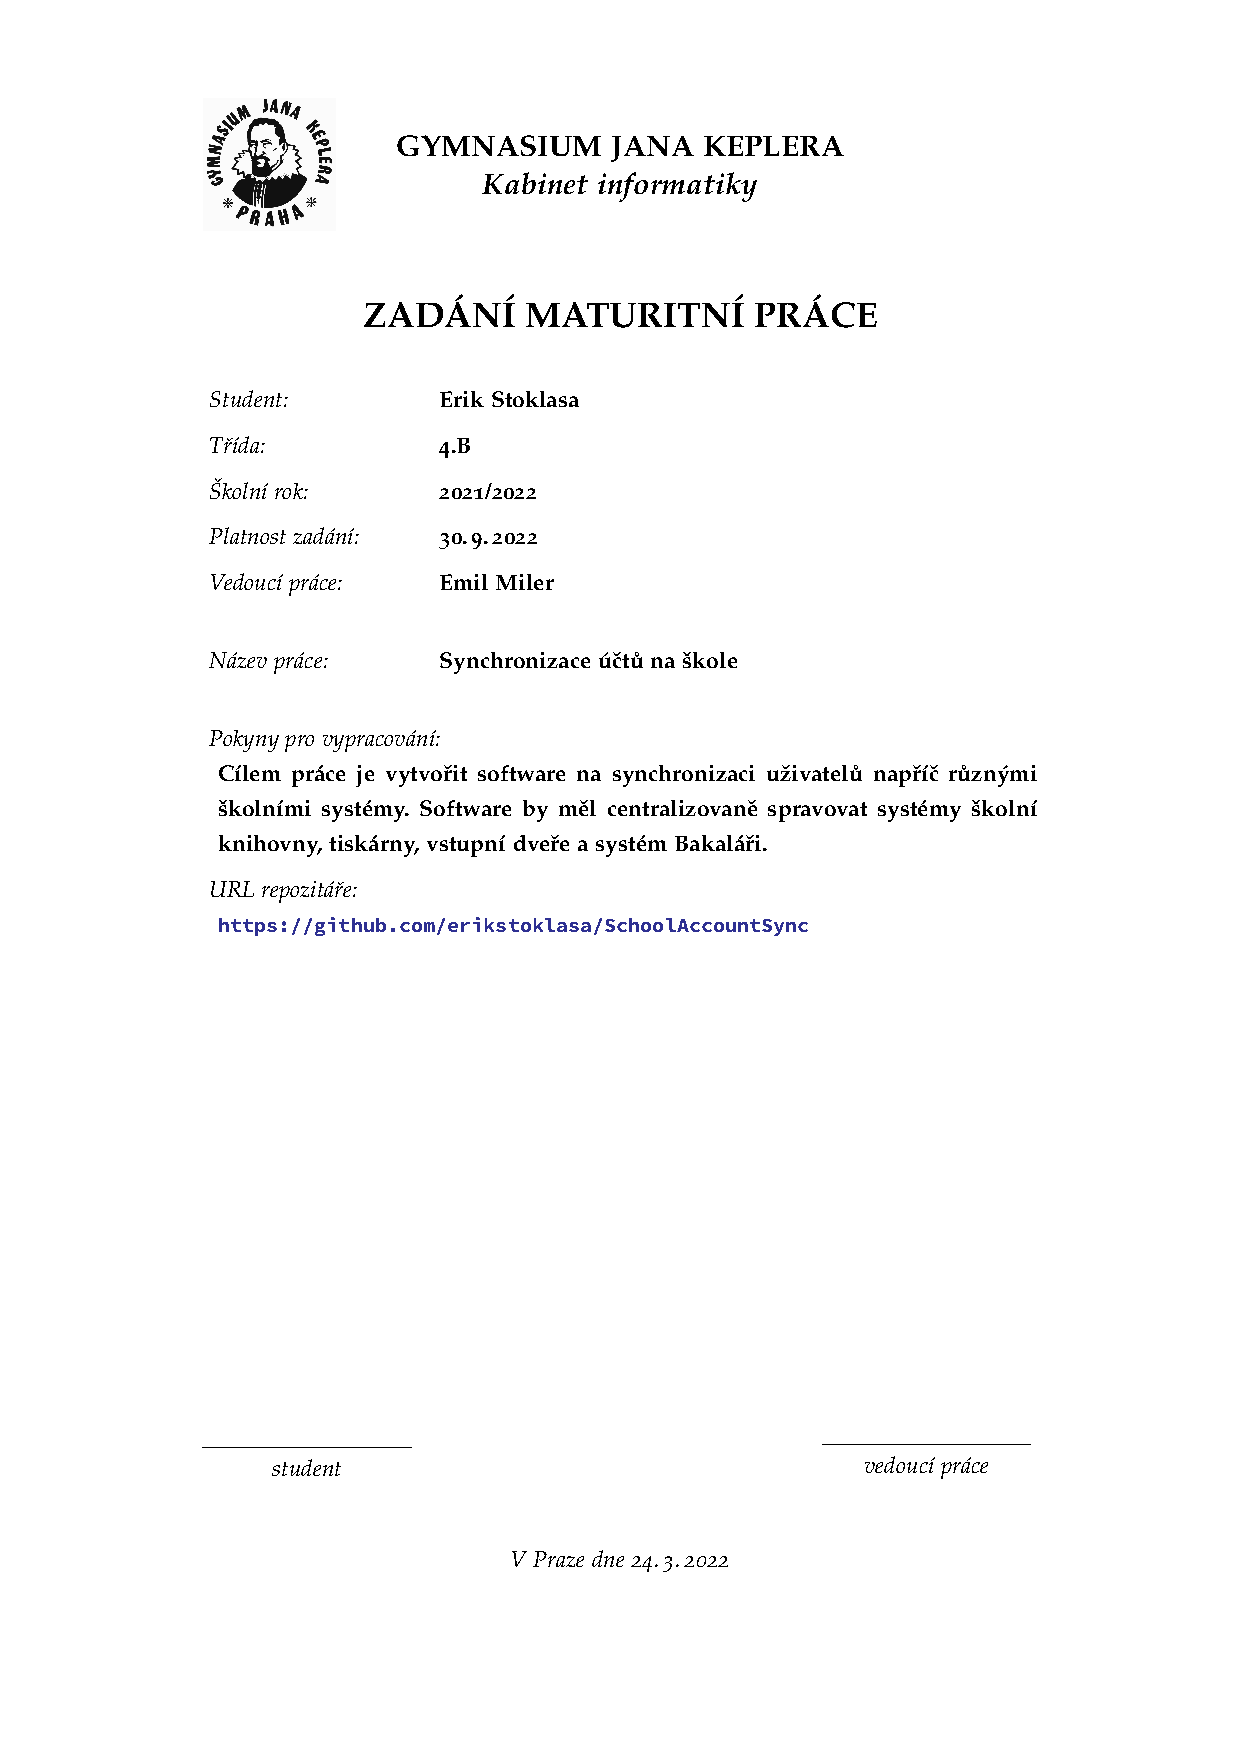
\includepdf[]{zadani.pdf}


%%% Strana s čestným prohlášením k bakalářské práci

\hypersetup{pageanchor=true}
\cleardoublepage
\vspace*{\fill}
\section*{Prohlášení}
\noindent
\Prohlaseni

\vspace{2cm}
\noindent
V Praze dne \today
\hspace*{\fill}\small{\AutorPrace}
\vspace{1cm}

%%% Poděkování
\openright
\vspace*{\fill}
\section*{Poděkování}
\noindent
\Podekovani
\vspace{1cm}


%%% Povinná informační strana bakalářské práce
\openright
\section*{Abstrakt}
\noindent
\Abstrakt
\subsection*{Klíčová slova}
\noindent
\KlicovaSlova

\vfill

\section*{Abstract}
\noindent
\AbstraktEN
\subsection*{Keywords}
\noindent
\KlicovaSlovaEN

\openright
\pagenumbering{arabic}

% Obsah
\setcounter{tocdepth}{2}
\tableofcontents

\chapter{Teoretická část}
\pagestyle{fancy}

Na Gymnáziu Jana Keplera se nachází mnoho školních systémů, které se starají o chod školy. Od knihovny, přes tiskárny, až po systém, který se stará o to, aby se do budovy dostali jen ti povolaní, tedy vstupní systém. Školní administrátor pak pro každého studenta musí vytvořit a spravovat účet v daném systému. Toto by nebylo problém, pokud by na škole bylo šedesát studentů, každopádně při škole, která je domovem pro přibližně 600 studentů je nutnost pracovat s vícero systémy velice časově náročná. Cílem této maturitní práce je vytvořit aplikaci, která tyto systémy spravuje a školní administrátor pak nemusí ztrácet svůj čas rutinní prací.


\chapter{Implementace}

Projekt byl zpracován v .NET 6, což je open source framework pro vytváření programů, které lze spustit na operačních systémech Windows, Linux a macOS. Byl použit programovací model Razor pages, který je alternativou ke klasickému MVC. Zároveň je celý projekt zabalený v kontaineru díky platformě Docker. Pro lokální databázi jsem zvolil PostgreSQL.

\section{.NET}
Framework .NET jsem si pro vypracování vybral, jelikož je oproti alternativám jako je třeba Node.js mnohem rychlejší a zároveň není závislý na platformě, na které bude spuštěn, což byla jedna z neznámých, při zakládání projektu. V této platformě se také dobře pracuje s daty díky LINQ, který jsem často používal. Zároveň na všechny databáze, na které jsem se potřeboval připojit, existovaly drivery, které jsem mohl využít. 
\section{Rešerše}
Tato část práce, musím bohužel říct, trvala přibližně stejně, ne-li více času, než celková implementace. Vyznat se v hordách tabulek školních systémů, na které se musím připojit, a které jsou zároveň pojmenované naprosto nesmyslnými názvy (ACCARD, AULEA, SYS0901, SYS0902, atd.) bylo pro mě naprosto ubíjející. Zároveň jsem měl ale naprostou radost, jakmile jsem po desítkách hodnin studování různých databázových tabulek přišel, jak opravdu fungují. Vše bylo ale nutné udělat ještě před tím, než začnu implementovat celý projekt.
\section{UX návrh}
Po rešerši jsem se pustil do designového návrhu projektu. Pracoval jsem v programu Figma, kde jsem si postupně vytvořil stránky dashboardu, konkrétního zobrazení studentů nebo zobrazení změn uživatelů. Často mi také pomáhalo si před implementací kódu jen ve Figmě načrtnout, jak by daná funkce měla vypadat, implementace byla pak jadnodušší a rychlejší.
\section{Napojení na systém tiskáren}
Tiskárny na Gymnáziu Jana Keplera fungují na databázovém serveru PostgreSQL. Pro napojení k tomuto serveru jsem využil knihovny Npgsql. Zároveň musím zmínit, že i přes velký počet tabulek v databázi (asi 150) dávalo smysl jejich pojmenování a tím pádem bylo pochopení struktury databáze mnohem jednodušší, než u ostatních školních systémů.
\section{Napojení na systém Bakaláři}
Ze systému Bakaláři stahuji data, je to tedy takový centrální systém pravdy. Pokud se něco v systému Bakaláři změní, bere se to za pravdivý údaj. Struktura tabulek v tomto systému byla také poměrně složitá, ale alespoň byly poměrně smysluplně pojemnovány.
\section{Napojení na systém knihovny}
Připojení na systém knihoven mi trvalo zprovoznit poměrně dlouho, jelikož se v průběhu mojí implementace změnil název databáze a zároveň se ze strany dodavatelské firmy systémz znepřístupnily určité tabulky. Bylo tedy možné naimplementovat jen jednoduchý způsob synchronizace se systémem, ale nebylo možné provést plnou synchronizaci.  
\section{Napojení na systém vstupních dveří}
Asi nejstarší a také nejsložitější systém, se kterým jsem musel kdy pracovat. Stovky tabulek s nesmyslnými názvy, které mezi sebou nemají ani žádné vztahy, obsahují duplikáty různých údajů na spoustě míst, tedy systém, se kterým je opravdu složité pracovat. Nakonec se mi povedlo zprovoznit jednoduchou synchronizaci, která dokáže aktualizovat RFID na základě lokálních dat.
\section{Budoucí vylepšení}
Potenciálních vylepšení v systému vidím opravdu hodně, například přidání autentifikace, tak aby mohla aplikace běžet na serveru a nejen lokálně na jednom počítači. Dalším z vylepšení je možné hledání kolizí v RFID záznamech, systém vás sice upozorní, jakmile se budete snažit synchronizovat s duplikovaným RFID, ale bylo by lepší uživatele upozornit ještě předtím.  

\chapter{Technická dokumentace}

Pro spuštění projektu je nutné vytvořit si PostgreSQL server, na kterém si musíte vytvořit tabulku dle souboru dbinit.sql. Dále je nutné spustit projekt s příkazem docker run. Přidáme environment variables, jak uvádí README soubor a aplikace je spuštěná.

\chapter*{Závěr}
\pagestyle{empty}
\addcontentsline{toc}{chapter}{Závěr}

Projekt splnil zadání v plné míře, dokáže spravovat dané systémy, i když bylo těžké s nimi někdy pracovat. V prámci projektu jsem se toho naučil opravdu hodně, hlavně s různými typy databází a zpracování dat.

%%% Seznam použité literatury
\nocite{timcorey}\nocite{npgsql}
\printbibliography[title={Seznam použité literatury},heading={bibintoc}]

%%% Přílohy k práci, existují-li. Každá příloha musí být alespoň jednou
%%% odkazována z vlastního textu práce. Přílohy se číslují.

%\part*{Přílohy}
%\appendix

\end{document}
